%
% instructions for "compiling":
%   latex main (first pass, also generates .aux file for bibtex)
%   bibtex main (generates .bbl file with bibliography)
%   latex main (second pass, incorporates bibliography)
%   latex main (do this if you still get messages about labels
%      having changed or missing references)
% to generate/view/print postscript:
%   dvips -o main.ps main 
%   gv main.ps (to view)
%   lpr main.ps (to print, or print from "gv")
% to generate/view/print PDF:
%   dvips -Pcmz -Ppdf -j0 -G0 -o main.ps main
%   ps2pdf main.ps main.pdf
%   acroread main.pdf (to view/print)
%   
\documentclass[11pt]{report}
\usepackage{amsmath}
\usepackage{algorithm}
\usepackage[noend]{algpseudocode}
\makeatletter
\def\BState{\State\hskip-\ALG@thistlm}
\makeatother
\usepackage{amssymb}
\usepackage{amsthm}
 
\theoremstyle{definition}
\newtheorem{definition}{Definition}[section]

\theoremstyle{lemma}
\newtheorem{lemma}{Lemma}[section]

\theoremstyle{corollary}
\newtheorem{corollary}{Corollary}[section]



\usepackage{graphicx}
\graphicspath{ {images/} }
% miscellaneous packages
% FIX THIS -- can add to or change, but these are useful
%
% uncomment the following if your input includes characters other than
% 7-bit ASCII (e.g., accented characters)
%\usepackage[utf8]{inputenc}
%
\usepackage{amsmath}
\usepackage{graphicx}
\usepackage{moreverb}
\usepackage{url}

% double spacing
\usepackage{setspace}
\doublespacing

% hyphenation
\usepackage[english]{babel}
\selectlanguage{english}

% allow more figures on a page
\setcounter{topnumber}{10}
\setcounter{bottomnumber}{10}
\setcounter{totalnumber}{10}
\setcounter{dbltopnumber}{10}
\def\topfraction{1.0}
\def\bottomfraction{1.0}
\def\textfraction{0.0}
\def\dbltopfraction{1.0}

% margins
%\usepackage[letterpaper,top=2.0in,bottom=1.5in,left=1.5in,right=1.0in]
%	{geometry}
\usepackage[top=2.0in,bottom=1.5in,left=1.5in,right=1.0in]{geometry}

% set up to put page numbers in header
\usepackage{fancyhdr}
\pagestyle{fancy}
\lhead{}
\chead{}
\rhead{\rm\thepage}
\lfoot{}
\cfoot{}
\rfoot{}
\renewcommand{\headrulewidth}{0pt}
\renewcommand{\footrulewidth}{0pt}

% author, title, and date
% FIX THIS
\newcommand{\theAuthor}{Your Name Here}
% FIX THIS -- but be sure to leave in \par if title might exceed
%   one line -- otherwise space between lines will be wrong
\newcommand{\theTitle}{Your Title Goes Here
	(It Can Be Really Really Really Really Long)\par}
% FIX THIS
\newcommand{\theDate}{April 1, 2005}

\newlength{\WidthOfX}
% do not set here -- set just before use so we get the right font size
%\settowidth{\WidthOfX}{X} 
\newenvironment{TitlePageList}
{\begin{list}{}{%
  \setlength\leftmargin{0pt}%
  \setlength\labelwidth{10pt}%
  \setlength\itemindent{0pt}%
  \let \makelabel\descriptionlabel%
}}
{\end{list}}

% FIX THIS -- can put additional macro definitions here

%----------------------------------------------------------------------

\begin{document}

\pagenumbering{gobble}

%
% spacing could probably be improved
%

\begin{center}

\bigskip

\begin{Large}
\textbf{\theTitle}
\end{Large}

\bigskip

\begin{large}
\theAuthor
\end{large}

\bigskip
\bigskip

\textbf{Abstract}

\end{center}

\noindent
% FIX THIS --- your abstract goes here.
A nice abstract goes here.



\clearpage
%
% spacing could probably be improved
%
\begin{center}

\bigskip

\begin{Large}
\textbf{Acknowledgments}
\end{Large}

\bigskip

\end{center}

%FIX THIS --- thank your advisor, etc., here.
Some acknowledgments go here.



\clearpage
\begin{singlespace}

\begin{center}

\textbf{\theTitle} 

\vspace*{\baselineskip}

\theAuthor 

\vspace*{\baselineskip}

A departmental senior thesis submitted to the \\
Department of Computer Science at Trinity University \\
in partial fulfillment of the requirements for graduation \\
with departmental honors. 

\vspace*{\baselineskip}

\theDate

\vfill

$\overline{\mbox{\rule{0in}{0.16in}Thesis Advisor~~~~~~~~~~~~~~~~~~~~~~~~~~}}$ 
\hfill
$\overline{\mbox{\rule{0in}{0.16in}Department Chair~~~~~~~~~~~~~~~~~~~~~~~~}}$ 

\vspace*{2\baselineskip}

$\overline{\mbox{\rule{0in}{0.16in}
~~~~~~~~Associate Vice President~~~~~~~~
}}$ \\
for \\
Academic Affairs

\end{center}

\vfill

\begin{small}

\settowidth{\WidthOfX}{X}

% FIX THIS comment/uncomment \item lines so correct box is checked
\noindent
Student Copyright Declaration: the author has selected the following
copyright provision:

\begin{TitlePageList}
%\item{[X]}
\item{[\hspace*{\WidthOfX}]}
This thesis is licensed under the
Creative Commons Attribution-NonCommercial-NoDerivs License, which
allows some noncommercial copying and distribution of the thesis,
given proper attribution.  To view a copy of this license, visit
\url{http://creativecommons.org/licenses/} or send a letter to Creative
Commons, 559 Nathan Abbott Way, Stanford, California 94305, USA.

%\item{[X]}
\item{[\hspace*{\WidthOfX}]}
This thesis is protected under the provisions of U.S. Code Title 17.
Any copying of this work other than ``fair use'' (17 USC 107)
is prohibited without the copyright holder's permission.

%\item{[X]}
\item{[\hspace*{\WidthOfX}]}
Other:

\end{TitlePageList}

\vspace*{2\baselineskip}

\noindent
% FIX THIS comment/uncomment \item lines so correct box is checked
Distribution options for digital thesis:

\begin{TitlePageList}

\item{[X]}
%\item{[\hspace*{\WidthOfX}]}
Open Access (full-text discoverable via search engines)

%\item{[X]}
\item{[\hspace*{\WidthOfX}]}
Restricted to campus viewing only (allow access only on the Trinity
University campus via \url{digitalcommons.trinity.edu})

\end{TitlePageList}

\end{small}

\end{singlespace}


\clearpage
%
% spacing could probably be improved
%

\begin{center}

\vfill

\begin{Huge}
\textbf{\theTitle}
\end{Huge}

\bigskip \bigskip \bigskip

\begin{huge}
\theAuthor
\end{huge}

\vfill

\end{center}


\tableofcontents
\listoftables
\listoffigures

\clearpage
\pagenumbering{arabic}

% FIX THIS -- one file per chapter is good but not required
\chapter{Introduction}


Researchers in both artificial intelligence (AI) and psychology share an interest in developing techniques for discerning the intentions of agents through observation \cite{schmidt:78,kautz:87}. AI researchers have referred to these types problems as \emph{goal recognition problems} (GR) or, more generally, \emph{plan recognition problems}~\cite{Sukthankar:14}. 
Plan and goal recognition models have many applications, both for cooporative and adversarial relationships between the agent in question and the party attempting to recognize their goal. Goal recognition has been used in designing software for personal assistants~\cite{oh:10,oh:11,oh:11b}; for
robots that interact with humans in cooporative work settings such as homes, offices, and hospitals~\cite{tavakkoli:07,kelley:12}; 
for intelligent tutoring systems that can recognize sources of confusion for a student based on
their interactions with the system~\cite{mcquiggan:08,johnson:10,lee:12,min:14}; and for security applications such as recognizing the goal of terrorists~\cite{jarvis:05}. 

\begin{figure}[h!]
\begin{center}

  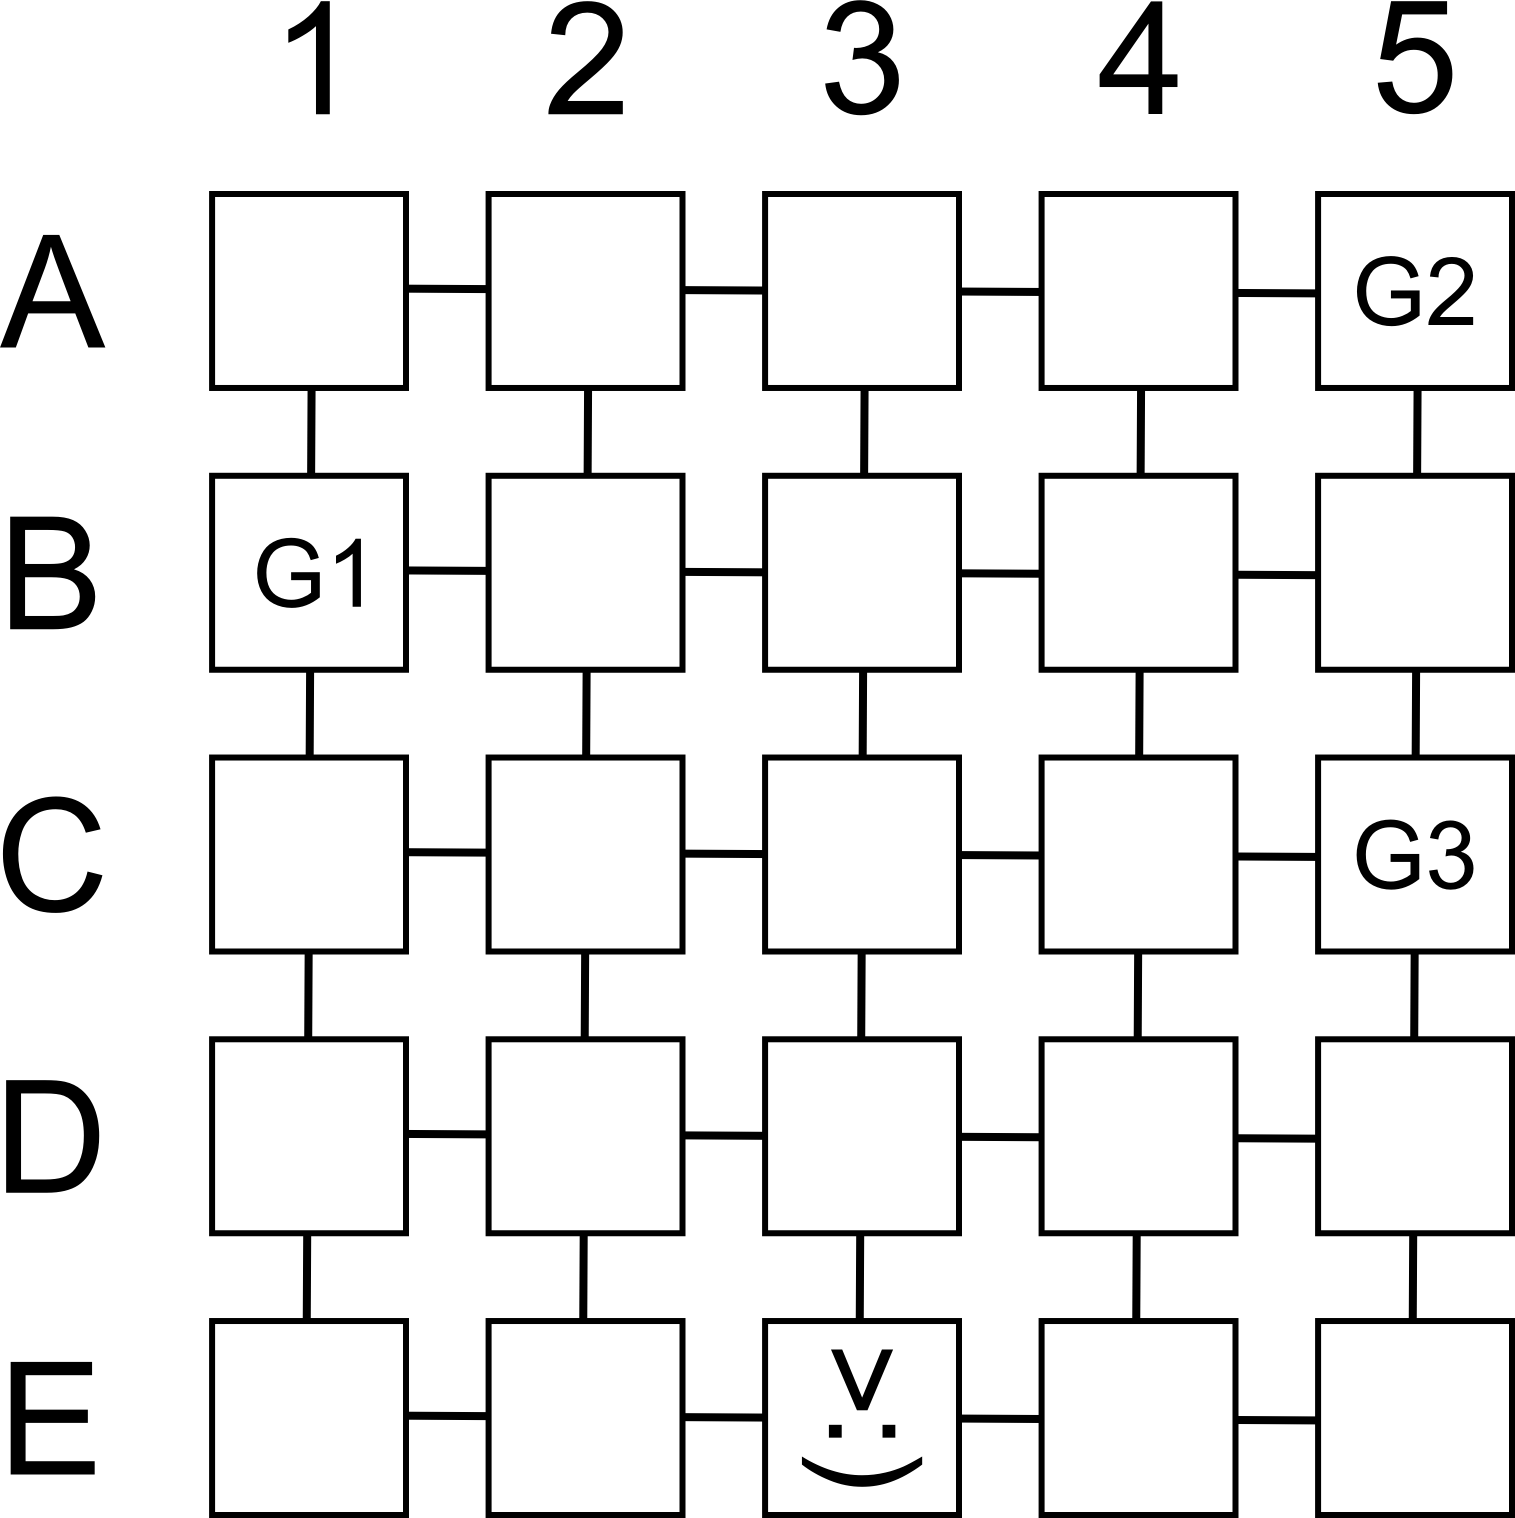
\includegraphics[scale=.15]{example1}
  \end{center}

  \caption{An Example Goal Recognition Problem.}
  \label{fig:example1}
\end{figure}


Goal recognition research focuses primarily on developing more effective, and more
efficient techniques for recognizing the goal of an agent through observing the agent's prior actions. Figure 1.1 illustrates a scenario in which a potentially malicious agent attempts to reach one of three goals. The agent in cell $E3$ can move to any adjacent cell on the graph. Cells $A5, B1,$ and $C5$, hold potential goal states for the agent. While the agent has a particular goal they want to reach, the observer is only aware of what goals the agent could potentially be working towards. In this scenario, a GR model could help an onlooker discern which goal the agent intends to reach.

Existing research into GR models has focused on partially strategic, or non strategic agents. While agents attempt to reach their secret goal at minimum cost, they do not explicitly reason about their interaction with observers.
When an observer's recognition of the agent's goal affects the agent in some way, 
then it is in the agent's best interest to be \emph{fully strategic}, and to
consider how their actions might affects the observer's recognition. 
As a result, the observer will need to take the agent's strategic reasoning into account when making decisions.

\subsection{Game-Theoretic Goal Recognition Problems in Security Domains}
Goal Recognition settings with strategic agents can model 
many real-world (physical and cyber) security scenarios between 
an adversary and a defender.  
In physical security domains, the adversary 
must make a sequence of 
physical movements to reach their target. 
In cyber security domains, this could be achieving a sequence of 
actions for necessary subgoals when carrying out an attack. 
In any case, the defender can benefit from recognizing the adversary's intended target in advance. 
Moving forward, we will take a game-theoretic approach to modeling such problems.

Consider the security scenario in Figure 1.1,
where an agent (i.e., a notorious art thief) wants to reach its intended target and carry out an some devilish action. Meanwhile we the observer must try to recognize the agent's goal as early as possible. 
Suppose that once we recognize the agent's goal, we can strengthen the agent's target to defend against the attack. 
The more time we have between recognition and the actual attack, the less successful the attack will be. 
In this scenario, the agent can not simply take the shortest path to its goal, since their intentions could quickly become clear to the observer.
At the same time, the agent should try to reach its goal in a reasonably short amount of time, 
as a very long path could allow the observer time to strengthen all the targets.
An optimal agent would need to explicitly reason about the tradeoffs 
between the cost of its path (e.g., path length) and the cost of an early discovery.

\subsection{Game-Theoretic Goal Recognition Design Problems in Security Domains}
So far we have discussed the defender's task in recognizing goals. 
However, the task could become extremely difficult in general. 
For instance, going back to our security example in Figure 1.1, 
if the agent moves up to $D3$, the observer cannot make any informed deductions. 
Unfortunately, if the agent moves along any one of the shortest paths to goal $G3$, then
throughout its entire path, we cannot deduce whether its goal is either $G2$ or $G3$!  Keren \emph{et al.} introduced the concept
of \emph{worst-case distinctiveness} ~\cite{keren:14}, the number of moves an agent can make before giving away their intentions.
This illustrates one of the challenges observers can face when tackling GR scenarios. There can exist large sequences of 
ambiguous observations which prevent the observer from picking out the correct target . 

\begin{figure}[h!]
\begin{center}

  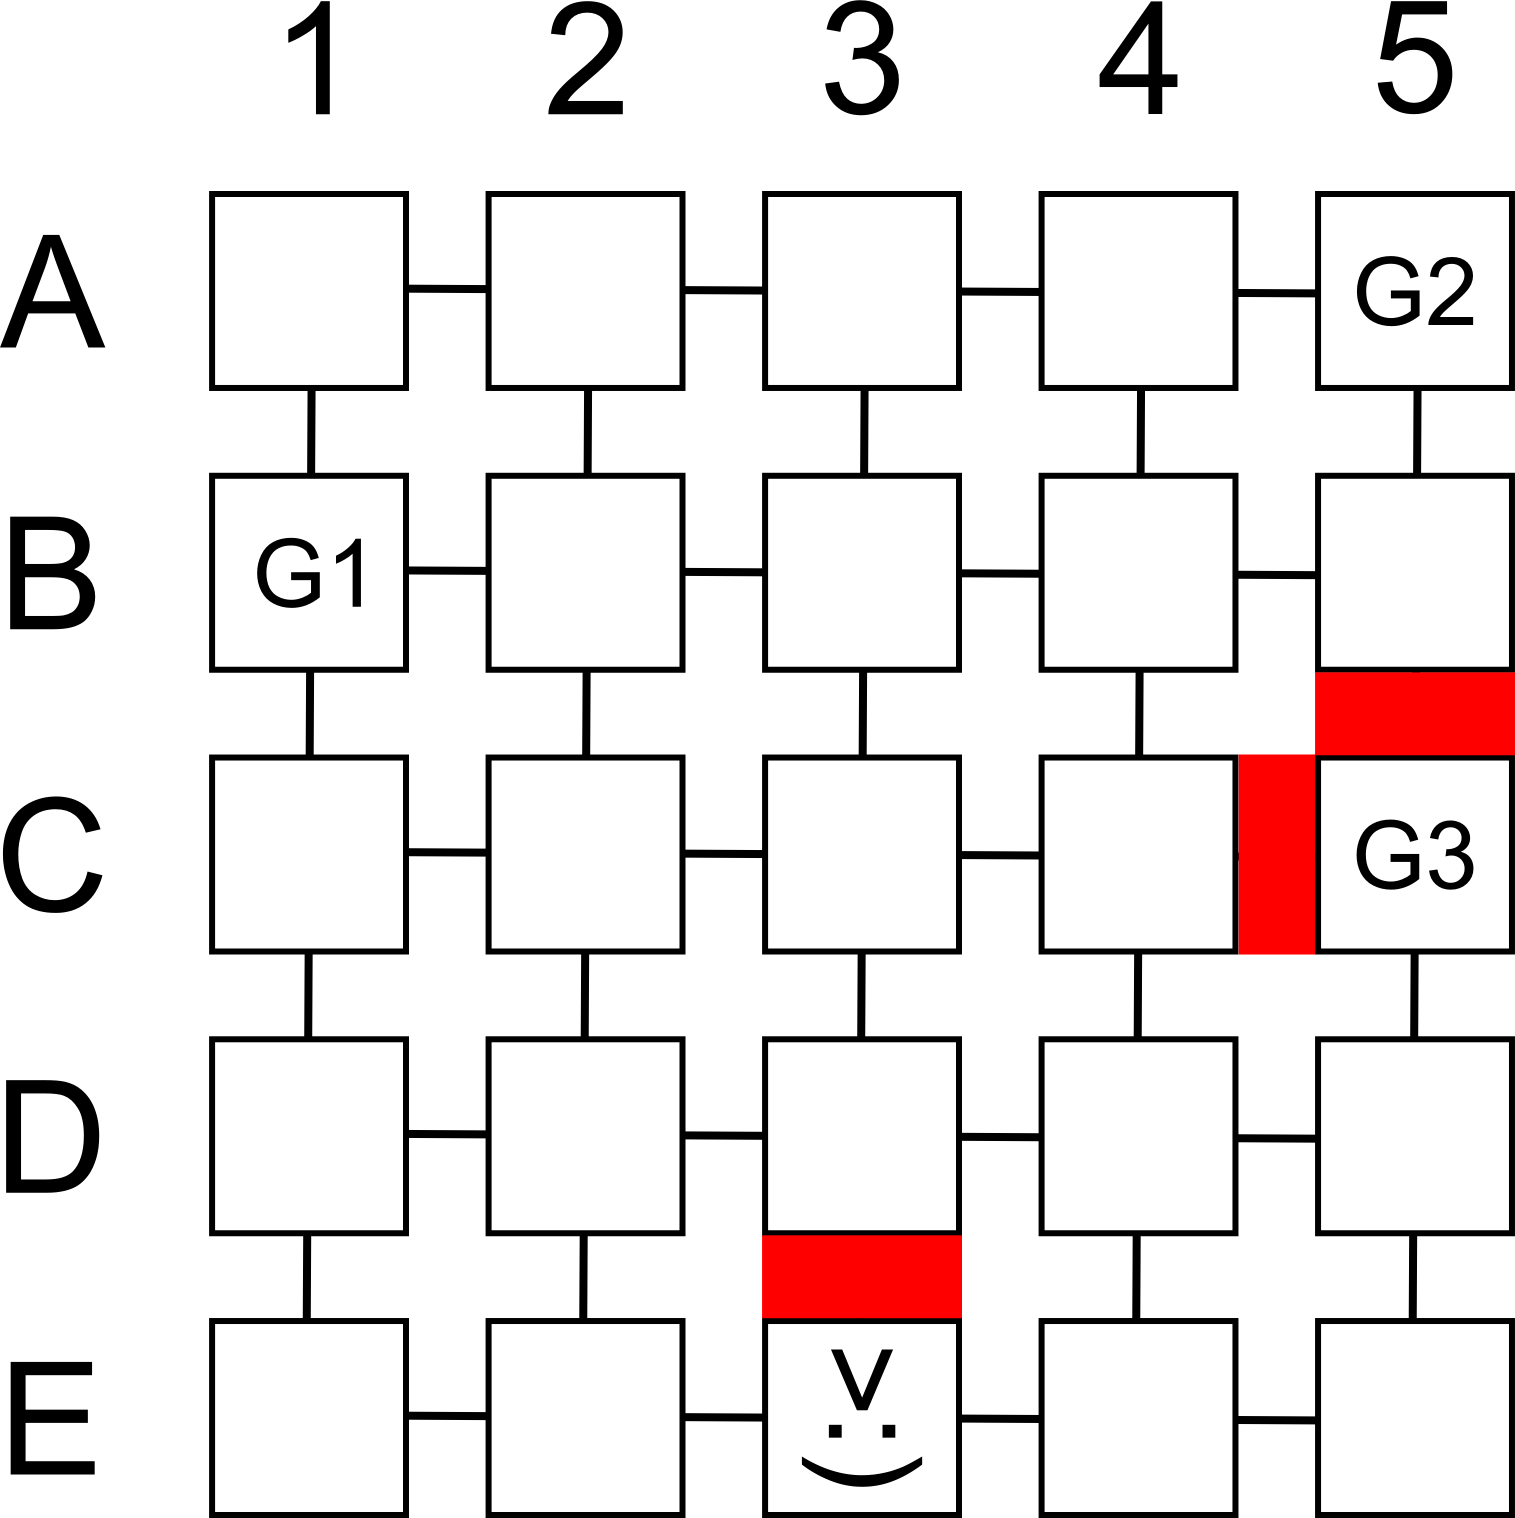
\includegraphics[scale=.15]{example2}
  \end{center}

  \caption{An Example Goal Recognition Design Problem with Blocked Edges.}
  \label{fig:example2}
\end{figure}


The work of \cite{keren:14,keren:15} proposed an orthogonal 
approach to \emph{modify the underlying environment of the agent}, in such a way that 
\emph{the agent is forced to reveal its goal as early as possible}. 
They call this problem the goal recognition design (GRD) problem. 
For example, if we block the actions $(E3, up), (C4, right)$, $(C5, up)$ in our example problem, 
where we use tuples $(s,a)$ to denote that action $a$ is blocked from cell $s$, then the agent can 
make at most 2 actions (i.e.,~right to E4 then up to D4) before its goal is conclusively revealed. 
Figure 1.2 shows the blocked actions for the previous example. 

%(perhaps with the help of roadblocks as in Figure \ref{example} (right)).
In addition to studying the Game Theoretic Goal Recognition problem (GTGR), we will also explore methods of solving the Game-Theoretic Goal Recognition Design  (GTGRD) problem, where the observer can modify the underlying environment (i.e., adding $K$ roadblocks)
in order to improve their odds of determining the agent's target.

\subsection{Related Work}

GR and its more general forms, plan recognition and intent recognition, have been extensively studied~\cite{Sukthankar:14} since their inception almost 40 years ago~\cite{schmidt:78}. Researchers have made significant progress within the last decade through synergistic integrations of techniques ranging from natural language processing~\cite{vilain:90,geib:07} to classical planning~\cite{ramirez:09,ramirez:10,ramirez:11} and deep learning~\cite{min:14}. The closest body of work to ours is the one that uses game-theoretic formulations, including an adversarial plan recognition model that is defined as an imperfect information two-player zero-sum game in extensive form~\cite{lisy:12}, 
a model where the game is over attack graphs~\cite{braynov:06}, 
and an extension that allows for stochastic action outcomes~\cite{guillarme:15}. 

GR has a long history and extensive literature, but the field of GRD is relatively new. Keren \emph{et al.} introduced the problem in their seminal paper~\cite{keren:14}, where they proposed a decision-theoretic STRIPS-based formulation of the problem. In the original GRD problem, the authors make several simplifying assumptions: (1) the observed agent is assumed to execute an optimal (i.e.,~cost-minimal) plan to its goal; (2) the actions of the agent are deterministic; and (3) the actions of the agent are fully observable. Since then, these assumptions have been independently relaxed, where agents can now execute boundedly-suboptimal plans~\cite{keren:15}, actions of the agents can be stochastic~\cite{wayllace:16}, and actions of the agents can be only partially observable~\cite{keren:16}. Further, aside from all the decision-theoretic approaches above, researchers have also modeled and solved the original GRD problem using answer set programming~\cite{son:16}. The key difference between these works and ours is that ours introduced a game-theoretic formulation that can more accurately capture interactions between the agent and the observer in security applications.  

\subsection{Contributions}
As a result of the strategic interaction in the GTGR and GTGRD scenarios, the cost-minimal plan (the solution concept in GR problem) 
and worst-case distinctiveness (the solution concept in GRD problem)
are no longer suitable solution concepts since they do not reflect the behavior of strategic agents.
Instead, our objective here is to formulate game-theoretic models of the agent's and observer's interactions 
under GR and GRD settings. 
More specifically, we will attempt to model GTGR and GRGRD settings as zero-sum stochastic games
with incomplete information where the adversary's target is unknown to the observer. 
%We propose to model GTGR and GRGRD settings as zero-sum stochastic games
%with incomplete information about the adversary's intended target. %(i.e., private information).
%The games are played on graphs where vertices are states and edges are adversary's actions.
For the GTGR setting,
we show that if the defender is restricted to playing only stationary strategies, 
the problem of computing optimal strategies (for both defender and adversary)
can be formulated and represented compactly as a linear program. We will also explore approaches to solving a partially observable variant of the GTGR setting in which the observer can only know the position of the adversary for certain states. We will perform experiments to determine if the observer can improve their performance with a non-stationary strategy.
For the GTGRD setting,
where the defender can choose $K$ edges to block at the start of the game, 
we formulate the problem of computing optimal strategies as a mixed integer program,
and present a heuristic algorithm
based on LP duality and greedy methods.
We perform experiments to show that our heuristic algorithm
achieves good performance (i.e., close to defender's optimal value) with better scalability
compared to the mixed-integer programming approach.

\section{Preliminary: stochastic games} \label{stochastic_games}
In our two-player zero-sum single-controller stochastic game $G$, 
(a) we have a finite set $S$ of states, 
and an initial state $s_0 \in S$, 
(b) given a state $s \in S$, a finite action set $J_{s}$ and $I=I_s$ 
for the first player and for the second player, respectively, 
(c) given a state $s \in S$ and $j \in J_s$, a single-controller transition function
$\chi(s, j)$ that deterministically maps the current state and action to a new state, 
%\footnote{Typically, the transition function depends on 
%both actions of the players and is mapped to some distribution over the states.}, 
and (d) given a state $s \in S$, $j \in J_s$, and $i \in I$, 
a reward function $r(s,i,j,\theta) \in \mathbb{R}$. 
Since this is a zero-sum game, without loss of generality, 
we define $r$ to be the reward for player 2 and 
the reward of player 1 is the negative reward of player 2. 
We consider two-player zero-sum single-controller stochastic game 
where player 2 has incomplete information. 
In particular, the game consists of a collection of zero-sum 
single-controller stochastic games $\{G_\theta\}_{\theta \in B}$ 
and a probability distribution $P \in \Delta(B)$ over $B$. 
For our setting, we assume that each stochastic game 
$G_\theta$ could have different reward function $r^\theta$, but 
all of the games $G_\theta's$ have the same sets of states, actions, and transition rules. 
The game is played in stages over some finite time. 
First, a game $G_\theta$ is drawn according to $P$. 
The first player is informed of $\theta$
while the second player does not know $\theta$. 
At each stage of game $t$ with current state $s_t \in S$, 
the first player selects $j_t \in J_s$ 
and the second player selects $i_t \in I$, 
and $s_{t+1}$ is reached according to $\chi(s_t, j_t)$.
%Typically, $j_t$, $i_t$, and $s_{t+1}$ are known to both players in the standard model \cite{..}.
However, we assume that player 1 does not know $o_t$, 
and both of the players do not know $r^\theta(s_t, i_t, j_t)$. Note that 
player 2 can infer the action of player 1 given the new state 
since our transition function is deterministic. Hence,
player 2 knows $j_t$, $i_t$, and $s_{t+1}$

The strategies of the players can be based on 
their own history of the previous states and strategies. 
In addition, player 1 can condition his strategies based 
on $\theta$. We consider finite timestep at most $T$. 
Let $h_t^1 = (s_0, j_0, s_1, j_1, ..., j_{t-1}, s_t)$ and 
$h_t^2 = (s_0, j_0, i_0, s_1, ...., j_{t-1}, i_{t-1}, s_t)$ 
to denote a possible history of length $t$ of player 1 and player 2
where $j_k \in J_{s_{k}}$ and $i_k \in I$ for $k=1, ..., t$. 
Let $H_{s_t}^1$ and $H_{s_t}^2$ be the set of all possible histories of length $t$ 
ended up at state $s_t$. 
Then, the sets of deterministic strategies for player 1 and player 2 are therefore 
$\prod_{t=0\le T, s_t \in S, h_{s_t}^1 \in H_{s_t}^1} J_{s_t}$ 
and $\prod_{t=0\le T, s_t \in S, h_{s_t}^2 \in H_{s_t}^2} I$ , respectively. 
Indeed, for each possible history, the players need to select some actions. 
Naturally, the players mixed strategies are distributions 
over the deterministic strategies. 

\begin{definition} \label{def:bhs}
Given $\theta \in B$, $0 \le t \le T$, $s_t \in S$,  $h_{s_t}^1 \in H_{s_t}^1$, 
%Given the sets $H^1$ and $H^2$ of histories, 
player 1's behavioral strategy $\sigma_1(\theta,$ $h_{s_t}^1, j_{s_t} )$ returns the probability 
of playing  $j_{s_t} \in J_{s_t}$ such that $\sum_{j_{s_t} \in J_{s_t}} \sigma_1(\theta, h_{s_t}^1, j_{s_t} ) = 1$. 
(Player 2's behavioral strategy $\sigma_2$ is defined similarly and does not depend on $\theta$). 
%$\sigma_1: B\times H^1 \to \Delta(A)$  
%and player 2's behavioral strategy is $\sigma_2: H^2 \to \Delta(O)$. 
\end{definition}

\begin{definition} \label{def:ss}
A behavioral strategy $\sigma$ is stationary if and only if it is independent of any timestep $t$
and  depends only on the current state 
(i.e., $\sigma_1(\theta,$ $h_{s}^1, j_{s} ) = \sigma_1(\theta,$ $\bar{h}_{s}^1, j_{s})$
%$\sigma_1(b,h) = \sigma_1(b,h')$ 
%for all $h, h'  \in H^1$  
such that $h_{s}^1$ and $\bar{h}_{s}^1$ have the same last state and
$\sigma_2$ can be defined similarly). 
\end{definition}

Given a sequence $\{(s_t,i_t,j_t)\}_{t=1}^T$ of actions and states, 
the total reward for player 2 is 
$r_T = \sum_{t=1}^T r^\theta(s_t,i_t,j_t)$. 
Thus, the expected reward 
$\gamma_T(P,s_0,\sigma_1,\sigma_2)$ $= \textbf{E}_{P,s_0,\sigma_1,\sigma_2}[r_T]$
is the expectation of $r_T$ over the set of stochastic games $\{G_\theta\}_{\theta \in B}$ 
%$B\times H^1$, and $H^2$ 
given the the fixed initial state $s_0$ under 
$P$, $\sigma_1$, and $\sigma_2$, respectively. 

\begin{definition}
The behavioral strategy $\sigma_2$ is a best response to $\sigma_1$ 
if and only if for all $\sigma_2'$, $\gamma_T(P,s_0,\sigma_1,\sigma_2) \ge \gamma_T(P,s_0,\sigma_1,\sigma_2')$. 
The behavioral strategy $\sigma_1$ is a best response to $\sigma_2$ 
if and only if for all $\sigma_1'$, $\gamma_T(P,s_0,\sigma_1,\sigma_2)$ $\le \gamma_T(P,s_0,\sigma_1',\sigma_2)$.
\end{definition}

For two-player zero-sum games, the standard solution concept is the max-min solution:
$\max_{\sigma_2} \min_{\sigma_1} \gamma_T(P,s_0,\sigma_1,\sigma_2) $.
%, where $x$ and $y$ are the observer's and the adversary's mixed strategies, respectively,
%and $u(x,y)$ is the expected utility to the observer given mixed strategies $x$ and $y$. 
One can also define min-max solution $ \min_{\sigma_1} \max_{\sigma_2} \gamma_T(P,s_0,\sigma_1,\sigma_2)$. 
For zero-sum games, the max-min value, min-max value, and 
Nash equilibrium values all coincide~\cite{fudenberg1991game}. 
For simultaneous-move games this can usually be solved by formulating a linear program. 
In this work, we will be focusing on computing the max-min solution. 

%\begin{definition}
%The behavioral strategies $\sigma_1$ and $\sigma_2$ are a Nash equilibrium 
%if and only if for all $\sigma_1'$ and $\sigma_2'$, 
%$\gamma_T(P,s_0,\sigma_1,\sigma_2) \ge \gamma_T(P,s_0,\sigma_1',\sigma_2)$ 
%and $\gamma_T(P,s_0,\sigma_1,\sigma_2)$ $\le \gamma_T(P,s_0,\sigma_1,\sigma_2')$. 
%\end{definition}


%[ADD our contributions and our plans???]



%
% FIX THIS -- remove/change, just some examples of things
%
\chapter{Game Model}
This chapter will introduce both the 
GTGR and GRGRD models. 

\subsection{Game-theoretic goal recognition model}\label{sec:game_basic}
Consider a deterministic environment such as the one in the introduction. 
We can model the environment with a graph 
in which the nodes correspond to the states  
and the edges connect neighboring states. 
Given the environment and the graph, as in many standard GR problems, 
the agent wants to plan out a sequence of moves (i.e., determining a path) 
to reach its target location of the graph.
The target location is unknown to the observer, and the observer's
goals are to identify the target location based on the observed sequence of moves 
and to make preventive measure to protect the target location. 
%In such scenario, it is clear that that the adversary's plan and
%the planner's move depend on each other. 
%To understand the behavior of the agents in a stable state, 
%We use game theory to model such scenario of high interdependence. 

We model this scenario as a two-player zero-sum game, between the agent/ adversary
and the observer. Given the graph $G = (L, E)$ of the environment, 
the adversary is interested in a set of potential targets $B \subseteq L$ 
and has a starting position $s_0 \in L \setminus B$. 
The adversary's aim is to attack a specific target $\theta \in B$, which 
is chosen at random according to some prior probability distribution $P$. 
The observer does not know the target $\theta$, and only the adversary knows its target $\theta$.  
However, the observer knows the set of possible targets $B$ and the adversary's starting position $s_0$. 
For any $s \in L$, we let $\nu(s)$ is the set of neighbors of $s$ in the graph $G$. 

The game is sequential and is played over several time-steps 
where both of the players move simultaneously. 
At each time-step, the observer selects a potential target in $B$ to protect, 
and the agent moves from its current position to a neighboring node.
With each time-step, the adversary and the observer will lose and gain a value $d$, respectively.
In addition, if the observer protects the correct target location $\theta$,
an additional value of $q$ will be added to the observer 
and subtracted from the adversary. The value $d$ allows us to incentivize quick play for the adversary, but can be set to $0$ such a penalty is not needed. Note that the value of $d$ should never be negative, since that would allow the adversary to wander the board endlessly, increasing their score to infinity.
The game ends when the attacker reaches its target $\theta$, 
a value of $u^{\theta}$ will be added to the adversary's overall score, and $u^{\theta}$ will be subtracted 
from the observer's overall score. 
Notice that during the play of the game, the adversary does not observe 
the observer's action(s), and the players do not know of their current scores. 

Because the adversary's moves may be stochastic in nature, and because the observer does not know the adversary's intended target, 
our setting is most naturally modeled as a 
\emph{stochastic game with incomplete information} 
as defined in Section \ref{stochastic_games}.
More specifically, the set of states is $L$ with an initial state $s_0$.
Given a state $s \in S$, $\nu(s)$ is the action set 
for the adversary and $B$ is the action set for the 
observer. Given a state $s \in S$ and $j \in \nu(s)$, 
the single-controller transition function $\chi(s,j) = j$. 
Indeed, the transition between states are controlled 
by the adversary only and is deterministic: From state $s$,
where $s\neq \theta$, given attacker action $j \in \nu(s)$,
the next state is $j$. %, where $\nu(s)$ is the set of neighbors of $s$. 
The state $\theta$ is terminal: Once reached, the game ends.
Given a state $s \in S$, $j \in \nu(s)$, and $i \in B$, 
%a reward function $r(s,i,j) \in \mathbb{R}$. 
%which is a multi-agent generalization of Markov decision (MDP) processes.
%Furthermore, the uncertainty of adversary's target in the system makes our game a stochastic game
%with incomplete information. 
%Formally, a given state $s$ in the game is solely comprised of the location of the attacker. 
%The action of the observer is denoted by $i\in B$ and the action of the adversary denoted by $j\in L$, 
we define the reward function $r^\theta(s,i,j) \equiv r(s, i, j, \theta)$ from the observer's point of view as
\begin{align}
r(s, i, j, \theta) = \left\{
        \begin{array}{ll}
            d & \quad j \neq \theta \textsl{ \& } i\neq \theta \\
            d+q & \quad j \neq \theta \textsl{ \& } i=\theta \\
            d-u^{\theta} & \quad j=\theta \textsl{ \& } i\neq \theta \\
           d+q-u^{\theta} & \quad j=\theta \textsl{ \& } i=\theta. \\
        \end{array}
    \right.
\end{align}
While, in theory, the game could go on forever if the adversary never reaches his target $\theta$, 
because of the per-timestep cost of $d$, any path of sufficient length for the adversary would be 
dominated by the strategy of taking the shortest path to $\theta$.
Eliminating these dominated strategies allows us to set a finite bound for the duration of the game. Even in games where the value of $d$ is set to 0, the defender could potentially play a uniformly random strategy that imposes a cost of $\frac{q}{| B |}$ per timestep. Therefore, an adversary strategy taking forever would achieve a value of $-\infty$ against the uniformly random defender strategy. In any Nash equilibrium the attacker will always reach their target in finite time.

We call this the game-theoretic goal recognition (GTGR) model. 
All of the definitions in Section \ref{stochastic_games} follow immediately from this game. 

\subsection{Game-theoretic goal recognition design model}
As mentioned in the introduction, we also consider the 
game-theoretic goal recognition design (GTGRD) model.
Formally, before the game starts, we allow the observer to block a subset 
of at most $K$ actions from the game. In our model, that corresponds to blocking at most $K$ edges from the graph.
In our game, blocking an edge does not prevent the adversary from taking the action,
but the adversary would incur a cost by taking that action. 
After placing the blocks, the game proceeds as described in Section \ref{sec:game_basic}.
\nocite{Dijkstra80}
\nocite{plop03-paper}


%
% FIX THIS -- remove/change, just some examples of things
%
\chapter{Computation}

\subsection{Game-theoretic goal recognition model}

With the game defined, we are interested in computing the solution of the game: 
What is the outcome of the game when both players behave rationally? 
Before defining rational behavior, we first need to discuss the set of strategies. In a sequential game, 
a pure strategy of a player is a deterministic mapping from the
current state and the player's observations/histories leading to the state, to an available action. For the adversary, such observations/histories include its own sequence 
of prior actions and its target $\theta$; 
the observer's observations/histories include 
the adversary's sequence of actions and the observer's sequence of actions.
A mixed strategy is a randomized strategy, specified by a probability distribution over the set of pure strategies.
The strategies are defined more formally in Section \ref{stochastic_games} and Definition \ref{def:bhs}.   
%For two-player zero-sum games, the standard solution concept is the max-min solution:
%$\max_x \min_y u(x,y)$, where $x$ and $y$ are the observer's and the adversary's mixed strategies, respectively,
%and $u(x,y)$ is the expected utility to the observer given mixed strategies $x$ and $y$. One can also define
%min-max solution $ \min_y\max_x u(x,y)$. 
%For zero-sum games, the max-min value, min-max value, and Nash equilibrium value all coincide~\cite{fudenberg1991game}. 

As mentioned earlier, we are interested in computing the max-min solution, 
which is equivalent to the max-min value, min-max value, and Nash equilibrium value  of the game. 
For simultaneous-move games this can usually be solved by formulating a linear program. 
However, for our sequential game, each pure strategy need to prescribe an action for each possible sequence of observations leading to that state and, as a result, the sets of pure strategies are exponential for both players. 

To overcome this computational challenge, we focus on \emph{stationary strategies}, 
which are strategies that depend only on the current 
state (for the adversary, also on $\theta$) and not on the history of observations (see Definition \ref{def:ss}).
While for stochastic games with complete information, it is known that there always exist an optimal solution that consists of stationary strategies~\cite{fudenberg1991game},
 it is an open question whether the same property holds for our setting, which is an incomplete-information game.
Nevertheless, there are some heuristic reasons
that stationary strategies are at least good approximately optimal solutions: The state (i.e., adversary's location) already capture a large amount of information about the strategic intention of the adversary.

%\vspace{-\medskipamount}
%\paragraph{Formulating the Linear Program.}
%\indent We borrow notation from \cite{....} on finite-step algorithms for single controller stochastic games. 
Restricting to stationary strategies,  randomized strategies now correspond to a mapping from state to a distribution over actions. We have thus reduced the dimension of the solution space from exponential to polynomial in the size of the graph.
Furthermore, our game exhibit the single-controller property: The state transitions are controlled by the adversary only. For complete information stochastic games with a single controller, a \emph{linear programming} (LP) formulation is known~\cite{Raghavan2003}. We adapt this LP formulation to our incomplete information setting.
 
We define $V(\theta, s)$ to be a variable that represents 
the expected payoff to the observer at state $s$ and with adversary's target begin $\theta$. 
We use $P(\theta)$ to denote the prior probability 
of $\theta \in B$ being the adversary's target such that $\sum_{\theta \in B} P(\theta) = 1$. 
The observer's objective is to find a (possibly randomized) strategy 
that maximizes his expected payoff given the prior distribution over the target set $B$, 
the moves of the adversary, and the adversary's starting location. 
The following linear program computes the utility of the observer in an max-min solution
assuming both players are playing a stationary strategy. 
\begin{align}
\!\!\!\!\max_{V, \{f_i(s)\}_{i,s}} \sum_{\theta}&P(\theta)V(\theta, s_{o}) \label{eq:game_obj}\\
V(\theta, s) &\leq \sum_{i \in B} r(s, i, j, \theta)f_{i}(s) + V(\theta, j) &\forall\theta\in B,\forall s \mid s\neq \theta, \forall j\in\nu(s)\label{eq:game_incentive}\\
V(\theta, s) &= 0 \quad &\mbox{when} \,\,\, s=\theta\label{eq:game_end}\\
\sum_{i} f_{i}(s) &= 1\quad &\forall s \label{eq:game_sum}\\
f_{i}(s) &\geq 0\quad &\forall s,i\label{eq:game_nonneg}
\end{align}
In the above linear program, \eqref{eq:game_obj} is the objective of the observer. 
The $f_{i}(s)$'s represent the probability of the observer taking an action $i \in B$ given the state $s$. 
To ensure that the probability distribution is well defined at each state of the games,
\eqref{eq:game_sum} and \eqref{eq:game_nonneg} impose the standard sum-equal-to-one and non-negative conditions on the probability of playing 
each action $i \in B$. The Bellman-like inequality \eqref{eq:game_incentive}
bounds the expected value for any state using 
expected values of next states plus the expected current reward, assuming the adversary will choose
the state transition that minimizes the observer's expected utility.
Finally, \eqref{eq:game_end} specifies the base condition when the adversary has reached their destination and the game ends. 
The size of the linear program is polynomial in the size of the graph. 
%While, in theory, the game could go on forever if the adversary never reaches his target $\theta$, 
%because of the per-timestep cost of $d$, any sufficiently long path for the adversary would be 
%dominated by the strategy of taking the shortest path to $\theta$. 
%Eliminating these dominated strategies allows us to set a finite bound for the duration of the game, 
%which grows linearly in the shortest distance to the target that is furthest away.

The solution of this linear program prescribes a randomized stationary strategy $f_i(s)$ 
for the observer and, from the dual solutions, one can compute a stationary strategy for the adversary.
In more detail, the dual linear program is
\begin{align}
\min &\sum_{s}t_s\label{eq:dual_obj}\\
t_s&\geq \sum_{\theta, j}\lambda^\theta_{s,j}r(s,i,j,\theta) &\forall s,i \label{eq:dual_incentive}\\
I_{s=s_0}P(\theta)+\sum_{s' \neq \theta: s\in \nu(s')}\lambda^\theta_{s',s} &=\sum_{j\in\nu(s)}\lambda^\theta_{s,j} &\forall\theta\in B,\forall s\neq \theta\label{eq:dual_flow}\\
\lambda^\theta_{s,j}&\geq 0    &\forall \theta,s,j
\end{align}
where $I_{s=s_0}$ is the indicator that equals 1 when $s=s_0$ and 0 otherwise.
The dual variables $\lambda^\theta_{s,j}$
can be interpreted as the probability that
adversary type $\theta$ takes the edge from $s$ to $j$.
These probabilities satisfies the flow conservation constraints \eqref{eq:dual_flow}: given $\theta$, the total flow into $s$ (the left hand side) is equal to the probability that type $\theta$ visits $s$, which should equal the total flow out of $s$ (the right hand side).
The variables $t_s$ can be interpreted as the 
contribution to defender's utility from state $s$, assuming that the defender is choosing an optimal action at each state (ensured by constraint \eqref{eq:dual_incentive}). 

Given the dual solutions $\lambda^\theta_{s,j}$, 
we can compute a stationary strategy for the adversary:
let $\pi(j|\theta,s)$ be the probability that the adversary type $\theta$ chooses $j$ at state $s$.
Then for all $\theta\in B$ and $s\neq\theta$, $\pi(j|\theta,s)=
\frac{\lambda^\theta_{s,j}}{\sum_{j'\in\nu(s)}\lambda^\theta_{s,j'}}$.
It is straightforward to verify that by playing the stationary strategy $\pi$, the adversary
type $\theta$ will visit each edge $(s,j)$ with probability
$\lambda^\theta_{s,j}$.

\begin{lemma}
Given a stationary strategy for the defender, 
there exists a best response strategy for the adversary that is also a stationary strategy.
\end{lemma}
\begin{proof}[Sketch]
Given a stationary defender strategy $f_i(s)$, each adversary type $\theta$ now faces a Markov Decision Process (MDP)
problem, which admits a stationary strategy as its optimal solution.
\end{proof} 

More specifically,
since the state transitions are deterministic and fully controlled by the adversary,
each type $\theta$ faces a problem of determining the shortest path from $s_0$ to $\theta$, 
with the cost of each edge $(s,j)$ as
$\sum_{i\in B}f_i(s) r(s,i,j,\theta)$.
Looking into the components of $r(s,i,j,\theta)$, since the adversary reward $u^\theta$ for reaching target $\theta$ occurs exactly once at the target $\theta$,
it can be canceled out and the problem is equivalent to the shortest path problem from $s_0$ to $\theta$ with
edge cost $d+f_\theta(s) q$. Since edge costs are nonnegative the shortest paths will not involve cycles.

What this lemma implies is that if the defender plays the stationary strategy prescribed by the LP \eqref{eq:game_obj}, the adversary cannot 
do better than the value of the LP by deviating to a non-stationary strategy.
\begin{corollary}
If the defender plays the stationary strategy $f_i(s)$
given by the solutions of LP $\eqref{eq:game_obj}$,
the adversary's stationary strategy $\pi$ as prescribed by
LP $\eqref{eq:dual_obj}$ is a best response, i.e., no
non-stationary strategies can achieve a better outcome for the adversary.
\end{corollary}

While it is still an open question whether the defender has an optimal strategy that is stationary,
we have shown that if we restrict to  stationary strategies for the defender, it is in the best interest of the adversary to also stick to stationary strategies and our LP \eqref{eq:game_obj} do not overestimate the value of the game. 

\subsection{Game-theoretic goal recognition design model}
One can solve this GTGRD problem by brute-force, i.e., try every subset of edges to block and then for each case solve the resulting LP. The time complexity of this approach grows exponentially in $K$. 
Instead, we can encode the choice of edge removal as integer variables added to the LP formulation, resulting in a mixed-integer program (MIP). For example, we could replace
\eqref{eq:game_incentive} with
\begin{align}
V(\theta, s) \leq \sum_{i \in B} r(s, i, j, \theta)f_{i}(s) + V(\theta, j) + M z(s, j) 
\label{eq:mip_incentive}
\end{align}
where $M$ is a positive number, and 
$z(s, j)$ is a 0-1 integer variable indicating whether
the action/edge from $s$ to $j$ is blocked.
M thus represents the penalty that the attacker incurs if he nevertheless chooses to take the edge from $s$ to $j$ while it is blocked. By making $M$ sufficiently large, we can make the actions of crossing a blocked edge dominated and therefore effectively removing the edges that we block.
We also add the constraint $\sum_{s,j} z(s,j) \leq K $.
%We implemented the MIP solution utilizing off-the-shelf MIP solvers, and conduct experiments to measure its runtime performance.
%We will also explore other algorithmic approaches, including adapting ideas from existing GRD literature such as pruning techniques that we have previous proposed for GRD and S-GRD~\cite{son:16,wayllace:16}.


\subsubsection{Dual-based greedy heuristic.}
The MIP approach scales exponentially in the worst case as the size of the graph and K grows.
 We propose a heuristic method for selecting edges to block.
 We first solve the LP for goal recognition and its dual.
In particular, we look at the dual variable 
$\lambda^\theta_{s,j}$ for the constraint \eqref{eq:game_incentive}.
 This dual has the standard interpretation as the \emph{shadow price}:
it is the rate of change to the objective if we infinitesimally relax
constraint \eqref{eq:game_incentive}.

 Looking at the MIP, in particular constraint \eqref{eq:mip_incentive}, we see that by blocking off an action from $s$ to $j$ we are effectively relaxing the corresponding LP constraints \eqref{eq:game_incentive} 
indexed by $\theta,s,j$ for all $\theta\in B$.
These are the adversary's incentive constraints for going from $s$ to $j$, for all adversary types $\theta$.

Utilizing the shadow price interpretation of the duals, the sum of the duals corresponding to the 
edge from $s$ to $j$: 
$\sum_{\theta\in B} \lambda^\theta_{s,j}$
 gives the rate of change to the objective (i.e. defender's expected utility) if the edge $(s,j)$ is blocked by an infinitesimal amount.
 Choosing the edge that maximizes this,
 $\arg \max_{s,j}\sum_{\theta\in B} \lambda^\theta_{s,j}$
 we get the maximum rate of increase of our utility.
 These rates of changes hold only when the amount of relaxation (i.e., $M$) is infinitesimal. However,
 in practice we can still use this as a heuristic for choosing edges to block.\footnote{Another perspective: from the previous section we see that $\lambda^\theta_{s,j}$ is the probability that adversary type $\theta$ traverses the edge $s,j$. 
 Then if the adversary and defender do not change their strategies after the edge $(s,j)$ is blocked, the defender would receive an additional utility of 
 $M\sum_{\theta\in B} \lambda^\theta_{s,j}$ from the adversary's penalty for crossing that edge.}

When $K > 1$, we could choose the $K$ edges with the highest dual sums.
 Alternatively, we can use a greedy approach:
pick one edge  with the maximum dual sum, 
place a block on the edge and solve the updated LP for goal recognition, and pick the next edge using the updated duals, and repeat.
In our experiments, the latter greedy approach consistently achieved significantly higher expected utilities than the former.
Intuitively, by re-solving the LP after adding each edge,
we get a more accurate picture of the adversary's 
adaptations to the blocked edges.
Whereas the rates of changes used by the former approach are only accurate when the adversary do not adapt at all to the blocked edges (see footnote 1).
Our greedy heuristic is summarized as follows.
\begin{itemize} 

\item for $i=1 \ldots K$:
\begin{itemize}
\item Solve LP \eqref{eq:game_obj}, updated with the current blocked edges. If edge $(s,j)$ blocked, the corresponding constraint \eqref{eq:game_incentive} indexed $s,j,\theta$ for all $\theta$ are modified so that $M$ is added to the right hand side.
Get the primal and dual solutions.
\item Take an edge $(s^*,j^*) \in\arg \max_{s,j}\sum_{\theta\in B} \lambda^\theta_{s,j}$,
and add it to the set of blocked edges.


\end{itemize}
\item return the set of blocked edges, and the primal solution of the final LP as the defender's stationary strategy. 
\end{itemize}
\nocite{Dijkstra80}
\nocite{plop03-paper}

%%
% FIX THIS -- remove/change, just some examples of things
%
\chapter{Example chapter}

Example chapter, with apologies to Alex Kolliopoulos,
from whose thesis the examples of math and tables were
borrowed.

\section{Examples of figures and tables}
\label{section:example-figtbl}

This section contains some words, plus
Figure~\ref{fig:xor} and 
Table~\ref{table:treepurpose}.

words, words, words, words,
words, words, words, words,
words, words, words, words,
words, words, words, words,
words, words, words, words,
words, words, words, words,
words, words, words, words,
words, words, words, words,

\begin{figure}[hbtp]
\begin{center}
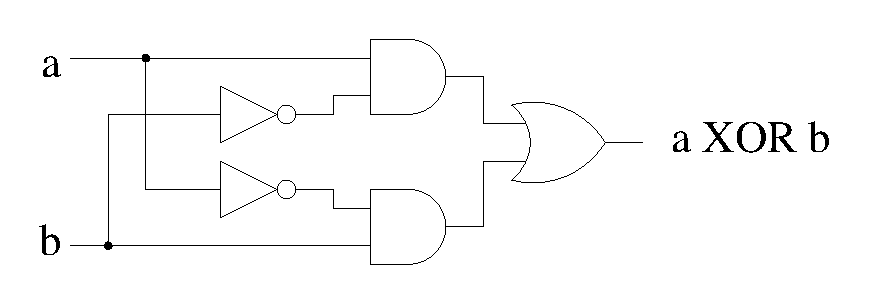
\includegraphics[width=0.5\textwidth]{xor}
\end{center}
\caption{An example figure.}
\label{fig:xor}
\end{figure}

words, words, words, words,
words, words, words, words,
words, words, words, words,
words, words, words, words,
words, words, words, words,
words, words, words, words,
words, words, words, words,
words, words, words, words,

\begin{table}[hbtp]
\begin{tabular}{|l|l|}
\hline 
\textbf{Trial 1} & Expanding a node to select a child\\
\hline
\textbf{Trial 3} & Selecting a node near the middle of a long, linear list\\
\hline
\textbf{Trial 4} & Selecting a node near the top of a long, linear list\\
\hline
\textbf{Trial 5} & Selecting a node near the bottom of a long, linear list\\
\hline
\textbf{Trial 6} & Scrolling and expanding folders in a large tree\\
\hline
\textbf{Trial 7} & Finding a node deep and near the bottom in a large tree\\
\hline
\textbf{Trial 8} & Finding a node near the top of a large tree\\
\hline
\end{tabular}
\caption{Purposes of each experimental trial.}
\label{table:treepurpose}
\end{table}
\section{Examples of math}
\label{section:example-math}

This section contains some math.
First, here's a set of equations.

\begin{eqnarray*}
y_p	&	=	&	\frac{y}{\sqrt{y^2+a^2}}, \\
y_p^2	&	=	&	\frac{y^2}{y^2+a^2}, \\
y_p^2	&	=	&	\frac{y^2+a^2-a^2}{y^2+a^2}, \\
y_p^2	&	=	&	1-\frac{a^2}{y^2+a^2}, \\
y_p^2-1	&	=	&	-\frac{a^2}{y^2+a^2}, \\
1-y_p^2	&	=	&	\frac{a^2}{y^2+a^2}.
\end{eqnarray*}

words, words, words, words,
words, words, words, words,
words, words, words, words,
words, words, words, words,
words, words, words, words,
words, words, words, words,
words, words, words, words,
words, words, words, words,

Now here's a numbered equation.

\begin{equation}
0 = 0 \label{eqn:example}
\end{equation}

\section{Examples of references}

% the "~" makes a no-line-breaks space
Section~\ref{section:example-figtbl} contains 
Figure~\ref{fig:xor} and
Table~\ref{table:treepurpose}.
Section~\ref{section:example-math} contains
Equation~(\ref{eqn:example}).
The sample bibliography file contains references to
a book \cite{gof-book} and a Web site \cite{MPI2}, plus some
other things.
% put in bibliography even though not referenced
\nocite{Dijkstra80}
\nocite{plop03-paper}


%
% FIX THIS -- remove/change, just some examples of things
%


\chapter{Partially Observable Environments}

\section{Introduction}
%this is how an image should look
%\includegraphics{universe}
Until now, both the GTGR and GTGRD models have given the observer full knowledge of the adversary's state for the entirety of the game. In real-world environments, observers may not have perfect information regarding the states and actions of an adversary. 

To accommodate for scenarios with incomplete information for the adversary, we introduce a partially observable variant of the GTGR scenario. In partially observable scenarios, the rules of the game remain largely unchanged, except for addition of “shadow states." The observer can not discern the current state of the adversary, while the adversary occupies a shadow state. When the adversary enters an observable portion of the graph, the observer will become aware of the adversary's position once more.

\begin{figure}[h!]
\begin{center}

  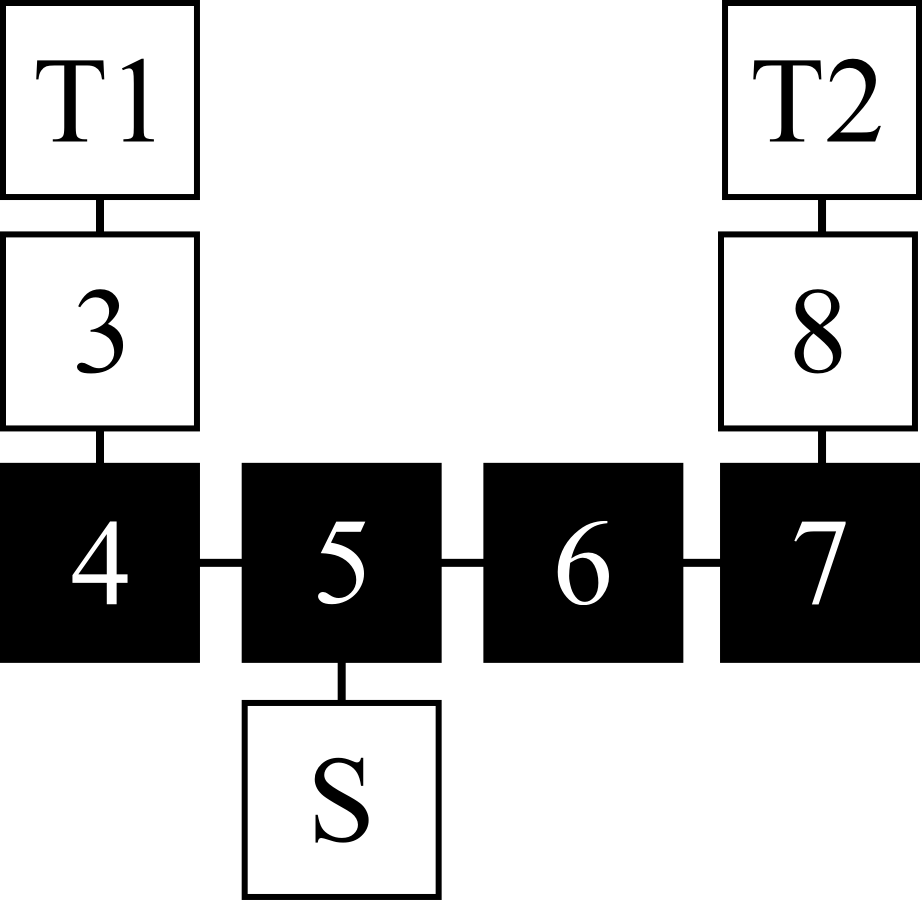
\includegraphics[scale=.15]{shadow1}
  \end{center}

  \caption{A partially observable graph.}
  \label{fig:shadow1}
\end{figure}

Figure~\ref{fig:shadow1} illustrates a partially observable environment. Visible states, in which the observer can see the adversary  white. Shadow states, in which the adversary is hidden from the observer, are black. The agent starts the game in state $S$. When the adversary moves to states $4$ ,$5$, $6$, or $7$, the observer is unable to determine their position until the adversary re-enters a visible portion of the graph.  
We will examine two solutions to the partially observable model, both of which involving linear programming. 

\section{The Whale Method}

The first method of solving partially observable environments, which we will call the "Whale Method," will utilize disjoint sets of shadow states. We call these sets of shadow states "shadow sets." We say that two shadow states belong to the same shadow set, if the adversary can travel between the two without entering an observable state.

\begin{figure}[h!]
\begin{center}

  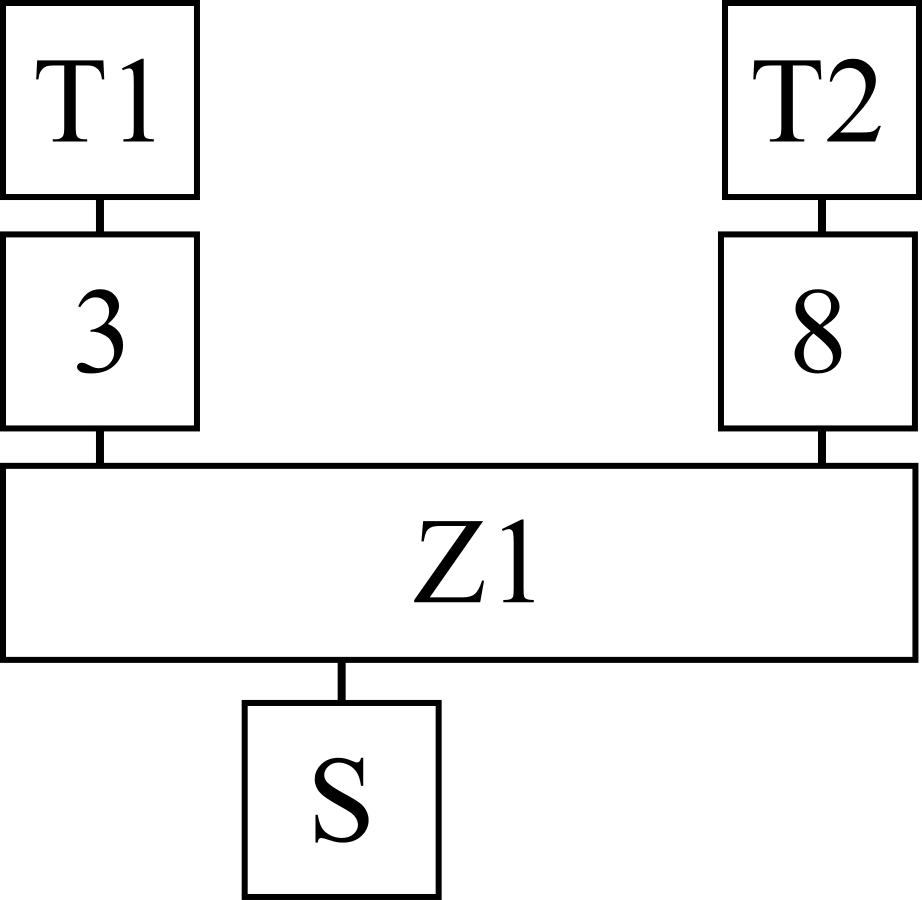
\includegraphics[scale=.15]{shadow2}
  \end{center}

  \caption{A partially observable graph with two shadow sets.}
  \label{fig:shadow2}
\end{figure}

The graph in Figure~\ref{fig:shadow2} has two disjoint shadow sets, one composed of states $2$ and $3$, the other composed of states $4$ and $5$. In using the Whale Method, the observer treats each shadow set a single state, which we will call a "whale state." We can identify the single shadow set in Figure~\ref{fig:shadow1}, composed of states $4$, $5$, $6$, and $7$. In using the Whale method, the observer treats each state in the shadow set as the same state. While the adversary may require several turns to travel among states $4$, $5$, $6$, and $7$, the adversary will act as if the has decided to remain stationary in the newly created state $W$ seen in Figure~\ref{fig:shadow3}

\begin{figure}[h!]
\begin{center}

  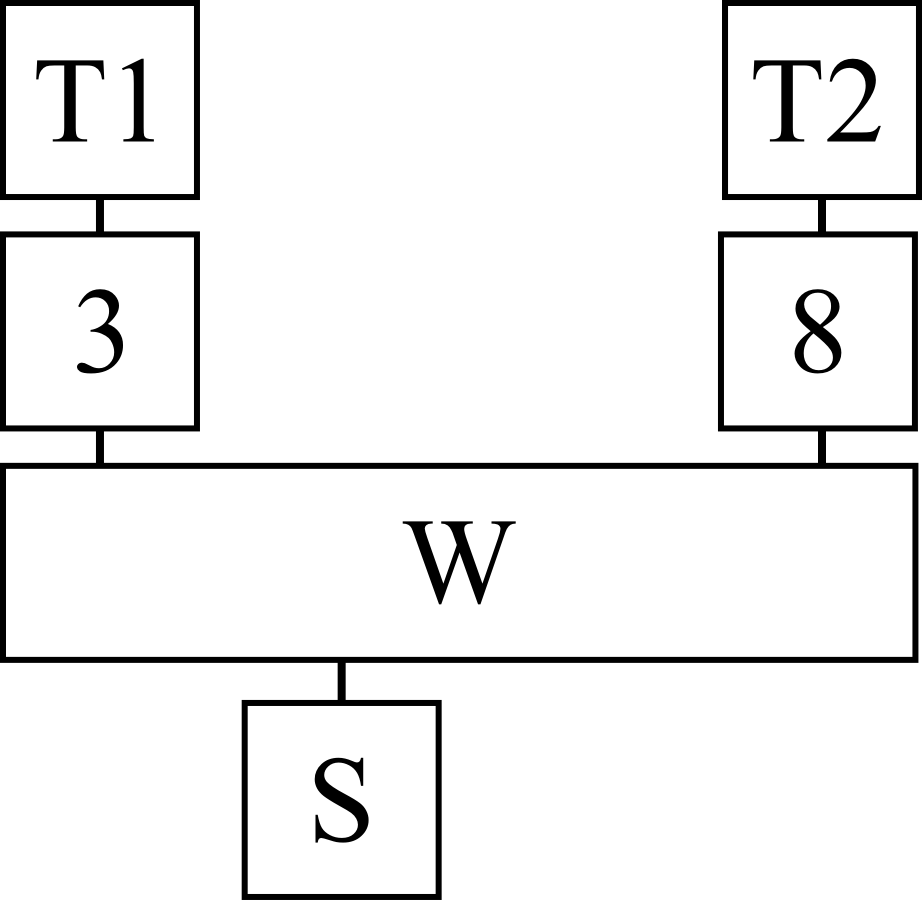
\includegraphics[scale=.15]{shadow3}
  \end{center}

  \caption{A partially observable graph with a single state in place of shadow states.}
  \label{fig:shadow3}
\end{figure}

We can add the following to the mixed integer program to accommodate for partially observable environments when using the Whale method.


\begin{equation}
V(\theta, s) \leq \sum_{i \in B} r(s, i, j, \theta)f_{i}(s) + V(\theta, j) \forall\theta\in B,\forall s \mid s\neq \theta, s\not\in H, \forall j\in\nu(s) \tag{3}
\end{equation}

\begin{equation}
V(\theta, s) \leq \sum_{i \in B} r(s, i, j, \theta)f_{w}(s) + V(\theta, j) \forall\theta\in B,\forall s \mid s\neq \theta, s\in H, \forall j\in\nu(s) \tag{3}
\end{equation}

\begin{equation}
\sum_{i} f_{i}(s) = 1\quad \forall s \tag{3}
\end{equation}

\begin{equation}
\sum_{w} f_{w}(s) = 1\quad \forall s \tag{3}
\end{equation}

\begin{equation}
f_{i}(s) \geq 0\quad \forall s,i\
\end{equation}

\begin{equation}
f_{w}(s) \geq 0\quad \forall s,w\
\end{equation}

We let $H$ denote the set of all shadow states, and $w$ denote the whale state the observer knows the adversary to be occupying. An observer action for any whale state $w$ is written as $f_{w}(s)$. These changes to the linear program require the observer to take the same action for each turn the adversary spends in a particular shadow set. The performance of the Whale method will be examined in a later section. 

\section{The Transmogrification Method}

When using the Whale method, the observer ignores some of the information available to them. The Whale method does not account for where the adversary entered a shadow set, or how long the adversary has remained hidden. The "Transmogrification Method" takes both of these pieces of information into account, by generating a fully observable environment from a partially observable environment. To do this, the observer must make some basic assumptions about the adversary's strategy. The following lemmas and corollary assume the agent is playing optimally against the observer's stationary strategy. 

\textbf{Lemma 2.} \textit{If the adversary's target does not lie within a shadow set, the adversary will eventually exit the shadow set.}

\textit{Proof (Sketch).} As mentioned previously, the game could theoretically go on forever. But because of the potential per-timestep cost of $d$ and the observer's predictions, any sufficiently long path for
the adversary would be dominated by the strategy of taking the shortest path to their target $\theta$. If the adversary never leaves the set of shadow states, then the game will go on forever. Thus, the adversary will eventually leave a shadow set. 

\textbf{Corollary 2.} \textit{An optimal agent occupying a state in a shadow set will take a shortest path to the exit state of their choosing.} 

\textit{Proof (Sketch).} We established that an optimal adversary in a shadow set must exit that shadow set. Each unnecessary turn the adversary spends in a shadow state invites the observer to guess their intended target. Thus, it is in the observer's interest to reach their chosen exit as quickly as possible.

With Corollary 2, the observer can generate a new graph to play on.

\begin{figure}[h!]
\begin{center}

  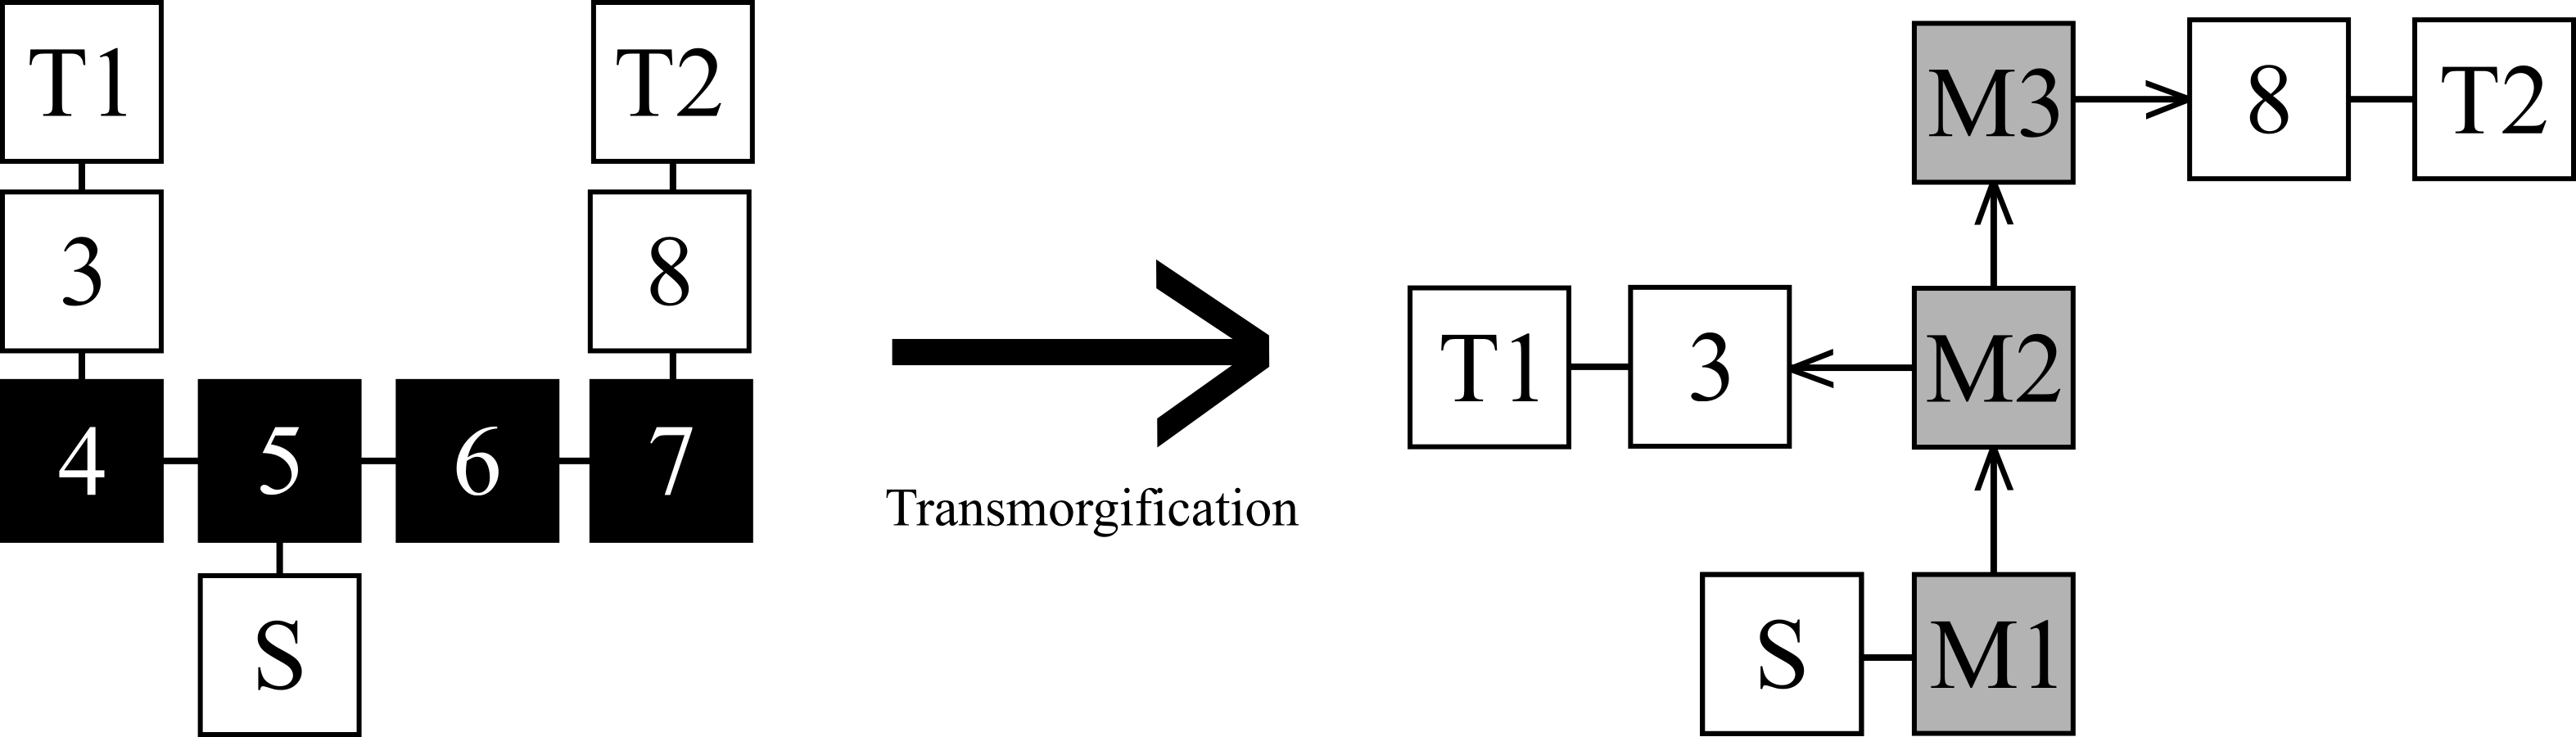
\includegraphics[scale=.15]{shadow4}
  \end{center}

  \caption{The partially observable environment from Figure~\ref{fig:shadow1} (left) transmogrified into an, fully observable graph.}
  
  \label{fig:shadow4}
\end{figure}

Figure~\ref{fig:shadow4} illustrates a transmogrified version of the graph from Figure ~\ref{fig:shadow1}. The grey nodes in the transmogrified graph are introduced to represent the number of turns the adversary has remained hidden from the observer. For instance, if the adversary has been hidden for two turns, then the observer would see the adversary as occupying state $M2$ in the transmogrified graph. Take note that the transmogrified graph now includes directed edges, because we are (hopefully) not dealing with a time traveling agent. To generate these graphs, we examine each shadow set. For each shadow set, we examine each "entrance state" connected by an edge to the shadow state. We then compute the shortest path between every two entrance states for that shadow state. By Corollary 2, we assume the length of the longest shortest path will be the maximum number of turns an optimal agent will spend within the shadow set. We then create create the same number of memory nodes with directed edges from one to the next (see states $M1, M2, M3$ from state $S$ in Figure ~\ref{fig:shadow4}). Then we create an edge from each entrance state, to the memory state corresponding to the length of the shortest path between the entrance state, and the original entrance state from which we spawned the memory states. For example, because a adversary would have to two shadow states on their journey from state $S$ to state $3$ in Figure ~\ref{fig:shadow1}, we connect state $M2$ to state $3$ in Figure ~\ref{fig:shadow4}. Note, that the post transmogrification graph in Figure ~\ref{fig:shadow4} is actually incomplete, because memory states have only been spawned from the entrance state $S$ and not from entrance states $3$ or $8$. Because an optimal agent has no reason to backtrack in this particular scenario, the memory nodes for $3$ and $8$ were omitted to keep the graph simple.

\begin{figure}[h!]
\begin{center}

  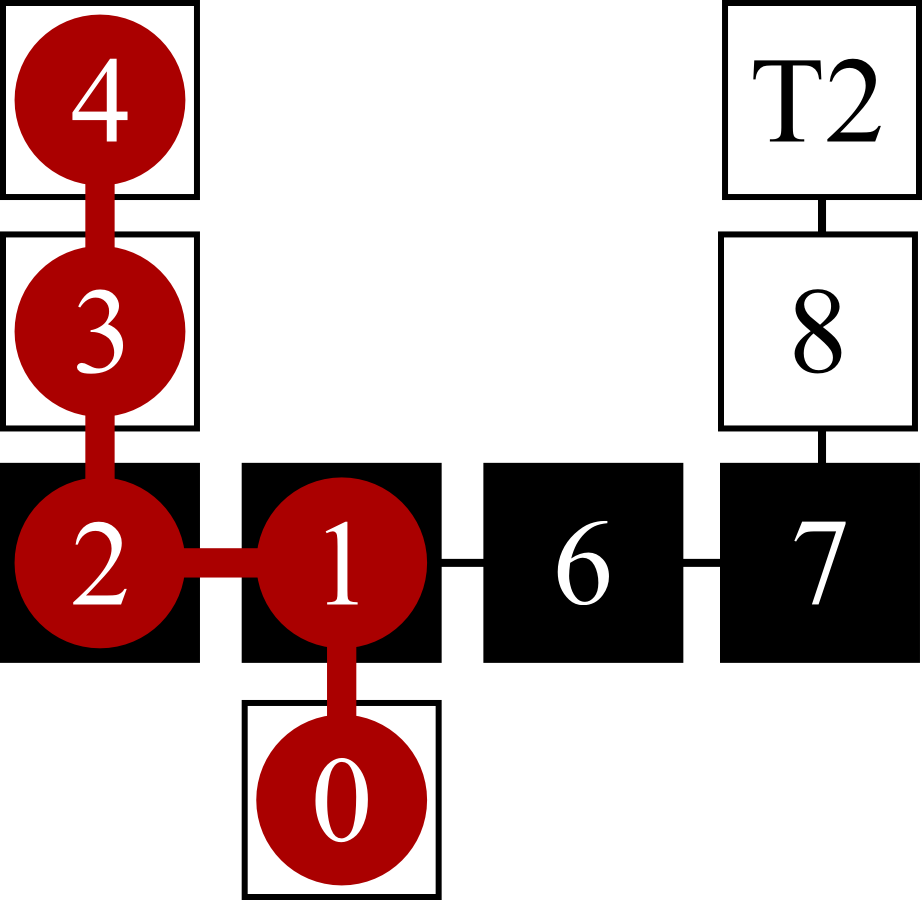
\includegraphics[scale=.15]{shadow5}
  \end{center}

  \caption{The adversary's path to target $T1$.}
  
  \label{fig:shadow5}
\end{figure}

Next, let us examine how a game might play out from the adversary's perspective.   Using the environment from Figure ~\ref{fig:shadow1}, let us assume the adversary was assigned target $T1$. Because the graph is rather limiting, the adversary takes the shortest path from starting state $S$ to the target $T1$. Figure ~\ref{fig:shadow5} illustrates the adversary's journey, each turn market with a red circle. Note that on turns $1$ and $2$, the observer would lose sight of the attacker until turn $3$. Now, let us examine what the same scenario would look like from the observer's prospective, when using the transmogrification method. 

\begin{figure}[h!]
\begin{center}

  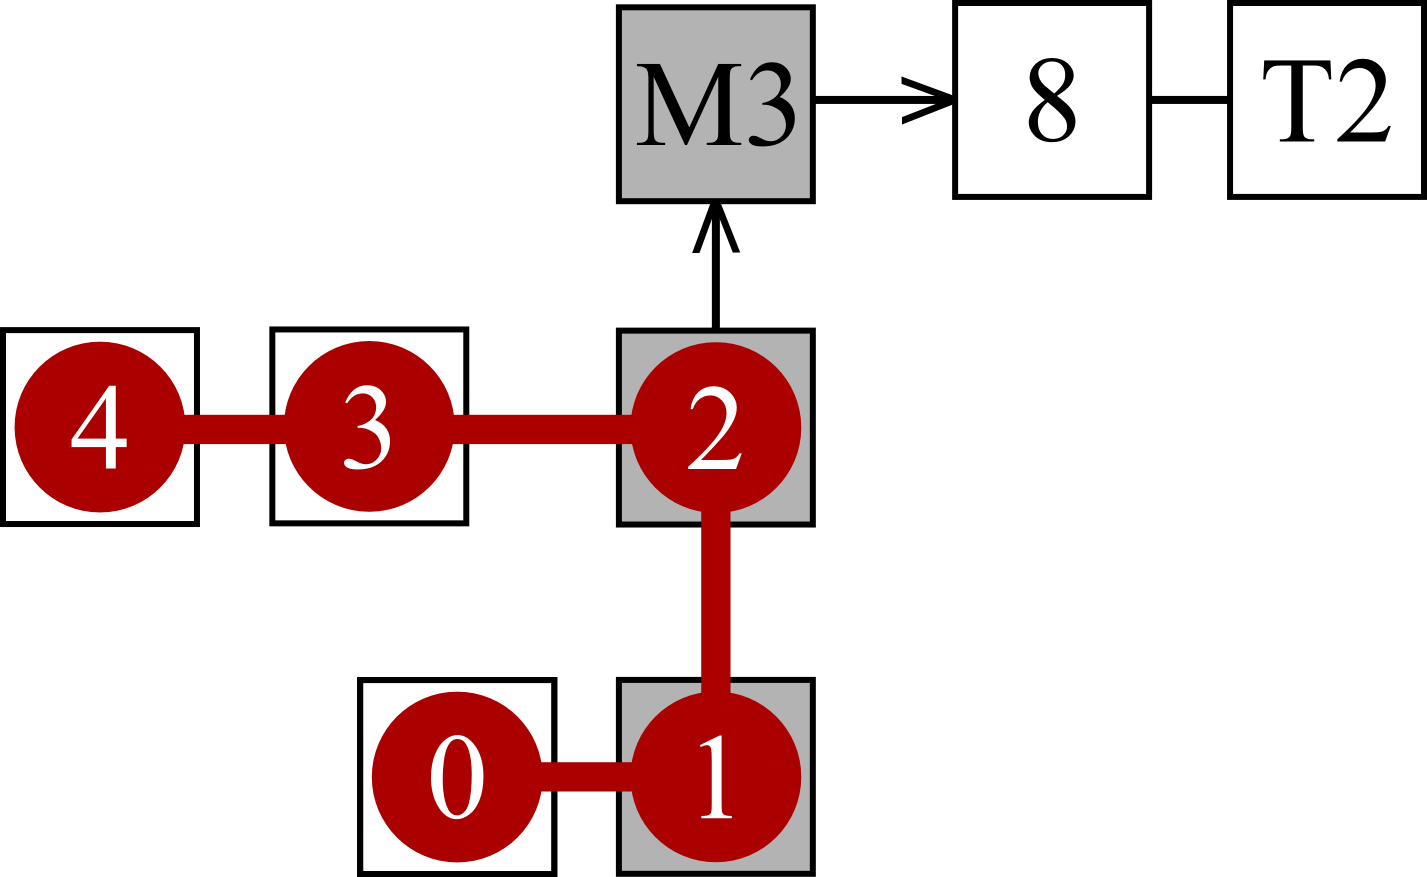
\includegraphics[scale=.15]{shadow6}
  \end{center}

  \caption{The adversary's path to $T1$ from the observer's perspective.}
  
  \label{fig:shadow6}
\end{figure}

Because the adversary takes two turns within the shadow set, the observer sees the adversary as moving from state $M1$ to state $M2$, before exiting the shadow set on turn 3. 

%explain code sample down below

\section{Experiments}

As with previous experiments, all tests were run on  a machine using OSX Yosemite version 10.10.5, with 16 GB of ram and a 2.3 GHz Intel Core i7 processor. First, we will use the simple example from Figure ~\ref{fig:shadow1} to compare the performance of the Whale, and Transmogrification methods. Additionally, we will compare the performance against a best case solution, in which we turn all shadow states into standard states. The best case solutions measures how the observer would perform if their strategy effectively negated the shadow states. Graphs were displayed using the Python NetworkX library. Arrowheads on directed edges were added manually for clarity. The starting state is displayed in green, target states are displayed in red, shadow states are displayed in purple, and default states are displayed in cyan.

\begin{figure}[h!]
\begin{center}

  \includegraphics[scale=.15]{test1}
  \end{center}

  \caption{A simple scenario using NetworkX.}
  
  \label{fig:test1}
\end{figure}

After transmogrifying the graph, the scenario becomes more complex, but allows the observer to play a fully observable game. There graph will no longer have any shadow states (purple). All states labeled with values greater than 1000 are nodes that have been added to represent turns hidden within the shadow set. Note that the graph in Figure ~\ref{fig:test2} will have more nodes than the previously seen illustration of the transmogrified graph in Figure ~\ref{fig:shadow4}, because we spawn memory states for every entry state, and not just the starting state. 

\begin{figure}[h!]
\begin{center}

  \includegraphics[scale=.15]{test2}
  \end{center}

  \caption{The transmogrified graph.}
  
  \label{fig:test2}
\end{figure}

For this game, the adversary is not penalized for timesteps taken. The reward for reaching the target is 0. The reward the observer receives for each correct guess was set to 1. The point value for each method at the end of the game equates to the number of correct guesses the observer can expect to make. At the start of the game, the adversary has a 75\% chance of being assigned target $1$, and a 25\% of being assigned target $2$.

\begin{table}[hbtp]
\begin{center}
\begin{tabular}{|l|l|}
\hline 
\textbf{No Shadow States} & 3.75 Correct Guesses\\
\hline
\textbf{Whale} & 3.25 Correct Guesses\\
\hline
\textbf{Transmogrification} & 3.50 Correct Guesses\\
\hline
\end{tabular}
\end{center}
\caption{Performance results from simple environment.}
\label{table:simpletable}
\end{table}

If a strategy were to effectively remove the shadow states from the board, the observer could expect to make 3.75 correct guesses over the course of the game. Thus, we could not expect the whale or transmogrification methods to perform any better. Using the whale methods, in which all shadow states a mushed together into one whale of a state, the observer can expect to make 3.25 correct guesses. While the transmogrification method does not allow the observer to effectively see through shadow states, the method still outperforms the whale method with a score of 3.50. Next, we will test these methods against each other in a more complex scenario.  

\begin{figure}[h!]
\begin{center}

  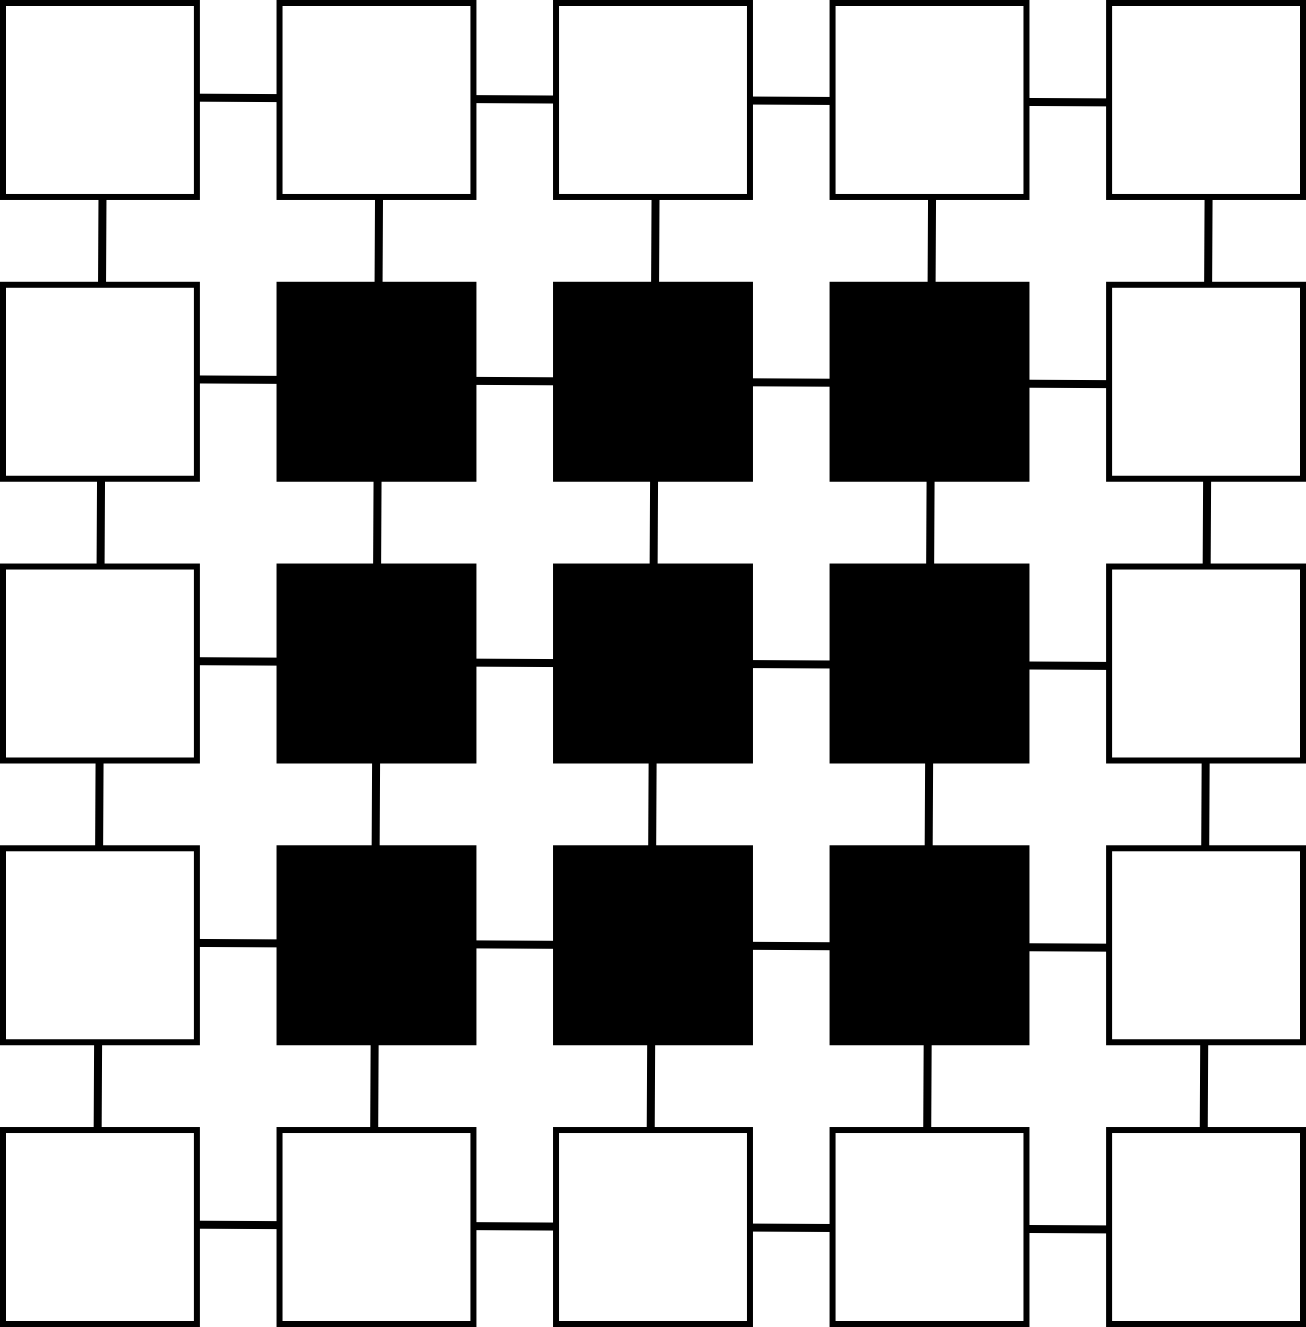
\includegraphics[scale=.15]{arena}
  \end{center}

  \caption{Complex testing environment.}
  
  \label{fig:arena}
\end{figure}

With the simple example out of the way, we move to a more complex environment which offers the adversary more freedom in approaching their target. For the next set of tests, we place the adversary starting state, and 3 potential targets on non-shadow states (marked in white) in Figure ~\ref{fig:arena}. We then create a random probability distribution, and solve the game with both methods. After ten-thousand iterations, the scores are averaged and compared. 

\begin{table}[hbtp]
\begin{center}
\begin{tabular}{|l|l|}
\hline 
\textbf{No Shadow States} & 2.65 Correct Guesses\\
\hline
\textbf{Whale} & 2.41 Correct Guesses\\
\hline
\textbf{Transmogrification} & 2.59 Correct Guesses\\
\hline
\end{tabular}
\end{center}
\caption{Average method performance in complex environment.}
\label{table:simpletable}
\end{table}

Though the transmogrification method does not yield what the observer could score without shadow states, it still outperforms the whale method.

\nocite{Dijkstra80}
\nocite{plop03-paper}


%
% FIX THIS -- remove/change, just some examples of things
%
\chapter{Conclusion}

\nocite{Dijkstra80}
\nocite{plop03-paper}
Motivated by the goal recognition (GR) 
and goal recognition design (GRD) problems 
in the artificial intelligence (AI) planning domain, 
we introduced and studied two natural variants of the 
GR and GRD problems with strategic agents. We considered game-theoretic (GT)
scenarios where a malicious adversary 
is aiming to cause damage to some target in an
(physical or virtual) environment monitored by a defender. We modeled GTGR and GTGRD settings as zero-sum stochastic games
with incomplete information regarding the adversary's intended target. We presented two solutions to the GTGRD setting. The mixed integer program gave optimal results when restricting the observer to stationary strategies. The dual-based greedy heuristic was capable of achieving similar performance with far better scalability. We also introduced a partially observable variant of the GTGR setting with imperfect information regarding the agent's location. The Whale method for approaching partially observable scenarios offered an inexpensive solution. The Transmogrification, though incredibly expensive offered better results. Though currently impractical, the Transmogrification method could become viable with the addition of selective pruning. 

% FIX THIS -- refs.bib is the bibtex file
\bibliography{refs}
\bibliographystyle{plain}

\appendix
% FIX THIS

\end{document}
